\documentclass{article}

\usepackage{amsmath,amssymb}
\usepackage{tikz}
\usepackage{pgfplots}
\usepackage{xcolor}
\usepackage{colortbl}
\usepackage[left=2.1cm,right=3.1cm,bottom=3cm,footskip=0.75cm,headsep=0.5cm]{geometry}
\usepackage{enumerate}
\usepackage{enumitem}
\usepackage{marvosym}
\usepackage{tabularx}
\usepackage[amsmath,thmmarks,standard]{ntheorem}
\usepackage{mathtools}

\usepackage[utf8]{inputenc}

\renewcommand*{\arraystretch}{1.4}
\newcommand{\E}{\mathbb{E}}

\newcolumntype{L}[1]{>{\raggedright\arraybackslash}p{#1}}
\newcolumntype{R}[1]{>{\raggedleft\arraybackslash}p{#1}}
\newcolumntype{C}[1]{>{\centering\let\newline\\\arraybackslash\hspace{0pt}}m{#1}}

\DeclareMathOperator{\tr}{tr}
\DeclareMathOperator{\Var}{Var}
\DeclareMathOperator{\Cov}{Cov}
\renewcommand{\E}{\mathbb{E}}

\newtheorem{thm}{Theorem}
\newtheorem{lem}{Lemma}

\title{\textbf{Einführung in die Logistik, Übung 5}}
\author{\textsc{Henry Haustein}}
\date{}

\begin{document}
	\maketitle
	
	\section*{Aufgabe 15}
	Vogel'sche Approximationsmethode
	\begin{center}
		\begin{tabular}{c|cccc|cc}
			& $j=1$ & $j=2$ & $j=3$ & $j=4$ & Angebot & Strafe \\
			\cline{1-6}
			$i=1$ & 0 & 1 & 1 & 4 & 5 & 1 \\
			$i=2$ & 1 & 0 & 1 & 2 \textbf{(2)} & 3 $\to$ 1 & 1 \\
			\rowcolor{blue!30}$i=3$ & 1 & 1 & 0 & 1 & 0 & \\
			\rowcolor{blue!30}$i=4$ & 4 & 2 & 1 & 0 & 0 & \\
			\cline{1-6}
			Nachfrage & 2 & 2 & 2 & 2 $\to$ 0 & & \\
			Strafe & 1 & 1 & 0 & \textcolor{red}{2} & &
		\end{tabular}
	\end{center}
	\begin{center}
		\begin{tabular}{c|cccc|cc}
			& $j=1$ & $j=2$ & $j=3$ & \cellcolor{blue!30}$j=4$ & Angebot & Strafe \\
			\cline{1-6}
			$i=1$ & 0 \textbf{(2)} & 1 & 1 & \cellcolor{blue!30}4 & 5 $\to$ 3 & \textcolor{red}{1} \\
			$i=2$ & 1 & 0 & 1 & \cellcolor{blue!30}2 \textbf{(2)} & 1 & 1 \\
			\rowcolor{blue!30}$i=3$ & 1 & 1 & 0 & \cellcolor{blue!30}1 & 0 & \\
			\rowcolor{blue!30}$i=4$ & 4 & 2 & 1 & \cellcolor{blue!30}0 & 0 & \\
			\cline{1-6}
			Nachfrage & 2 $\to$ 0 & 2 & 2 & \cellcolor{blue!30}0 & & \\
			Strafe & 1 & 1 & 0 & \cellcolor{blue!30} & &
		\end{tabular}
	\end{center}
	\begin{center}
		\begin{tabular}{c|cccc|cc}
			& \cellcolor{blue!30}$j=1$ & $j=2$ & $j=3$ & \cellcolor{blue!30}$j=4$ & Angebot & Strafe \\
			\cline{1-6}
			$i=1$ & \cellcolor{blue!30}0 \textbf{(2)} & 1 & 1 & \cellcolor{blue!30}4 & 3 & 0 \\
			$i=2$ & \cellcolor{blue!30}1 & 0 \textbf{(1)} & 1 & \cellcolor{blue!30}2 \textbf{(2)} & 1 $\to$ 0 & \textcolor{red}{1} \\
			\rowcolor{blue!30}$i=3$ & \cellcolor{blue!30}1 & 1 & 0 & \cellcolor{blue!30}1 & 0 & \\
			\rowcolor{blue!30}$i=4$ & \cellcolor{blue!30}4 & 2 & 1 & \cellcolor{blue!30}0 & 0 & \\
			\cline{1-6}
			Nachfrage & \cellcolor{blue!30}0 & 2 $\to$ 1 & 2 & \cellcolor{blue!30}0 & & \\
			Strafe & \cellcolor{blue!30} & 1 & 0 & \cellcolor{blue!30} & &
		\end{tabular}
	\end{center}
	\begin{center}
		\begin{tabular}{c|cccc|cc}
			& \cellcolor{blue!30}$j=1$ & $j=2$ & $j=3$ & \cellcolor{blue!30}$j=4$ & Angebot & Strafe \\
			\cline{1-6}
			$i=1$ & \cellcolor{blue!30}0 \textbf{(2)} & 1 \textbf{(1)} & 1 \textbf{(2)} & \cellcolor{blue!30}4 & 3 $\to$ 0 & \\
			\rowcolor{blue!30}$i=2$ & \cellcolor{blue!30}1 & 0 \textbf{(1)} & 1 & \cellcolor{blue!30}2 \textbf{(2)} & 1 $\to$ 0 & \\
			\rowcolor{blue!30}$i=3$ & \cellcolor{blue!30}1 & 1 & 0 & \cellcolor{blue!30}1 & 0 & \\
			\rowcolor{blue!30}$i=4$ & \cellcolor{blue!30}4 & 2 & 1 & \cellcolor{blue!30}0 & 0 & \\
			\cline{1-6}
			Nachfrage & \cellcolor{blue!30}0 & 1 $\to$ 0 & 2 $\to$ 0 & \cellcolor{blue!30}0 & & \\
			Strafe & \cellcolor{blue!30} & & & \cellcolor{blue!30} & &
		\end{tabular}
	\end{center}
	Gesamtkosten: $2\cdot 0 + 1\cdot 1 + 2\cdot 1 + 1\cdot 0 + 2\cdot 2 = 7$.

	\section*{Aufgabe 16}
	Vogel'sche Approximationsmethode
	\begin{center}
		\begin{tabular}{c|cccc|cc}
			& F & HH & K & M & Angebot & Strafe \\
			\cline{1-6}
			F & 0 \textbf{(2)} & 520 & 180 & 420 & 3 $\to$ 1 & \textcolor{red}{180} \\
			KA & 140 & 640 & 320 & 280 & 3 & 140 \\
			S & 210 & 700 & 390 & 210 & 3 & 0 \\
			\cline{1-6}
			Nachfrage & 2 $\to$ 0 & 2 & 3 & 2 & & \\
			Strafe & 140 & 120 & 140 & 70 & & 
		\end{tabular}
	\end{center}
	\begin{center}
		\begin{tabular}{c|cccc|cc}
			& \cellcolor{blue!30}F & HH & K & M & Angebot & Strafe \\
			\cline{1-6}
			F & \cellcolor{blue!30}0 \textbf{(2)} & 520 & 180 \textbf{(1)} & 420 & 1 $\to$ 0 & \textcolor{red}{240} \\
			KA & \cellcolor{blue!30}140 & 640 & 320 & 280 & 3 & 40 \\
			S & \cellcolor{blue!30}210 & 700 & 390 & 210 & 3 & 180 \\
			\cline{1-6}
			Nachfrage & \cellcolor{blue!30}0 & 2 & 3 $\to$ 2 & 2 & & \\
			Strafe & \cellcolor{blue!30} & 120 & 140 & 70 & & 
		\end{tabular}
	\end{center}
	\begin{center}
		\begin{tabular}{c|cccc|cc}
			& \cellcolor{blue!30}F & HH & K & M & Angebot & Strafe \\
			\cline{1-6}
			\rowcolor{blue!30}F & \cellcolor{blue!30}0 \textbf{(2)} & 520 & 180 \textbf{(1)} & 420 & 0 & \\
			KA & \cellcolor{blue!30}140 & 640 & 320 & 280 & 3 & 40 \\
			S & \cellcolor{blue!30}210 & 700 & 390 & 210 \textbf{(2)} & 3 $\to$ 1 & \textcolor{red}{180} \\
			\cline{1-6}
			Nachfrage & \cellcolor{blue!30}0 & 2 & 2 & 2 $\to$ 0 & & \\
			Strafe & \cellcolor{blue!30} & 60 & 70 & 70 & & 
		\end{tabular}
	\end{center}
	\begin{center}
		\begin{tabular}{c|cccc|cc}
			& \cellcolor{blue!30}F & HH & K & \cellcolor{blue!30}M & Angebot & Strafe \\
			\cline{1-6}
			\rowcolor{blue!30}F & \cellcolor{blue!30}0 \textbf{(2)} & 520 & 180 \textbf{(1)} & \cellcolor{blue!30}420 & 0 & \\
			KA & \cellcolor{blue!30}140 & 640 & 320 \textbf{(2)} & \cellcolor{blue!30}280 & 3 $\to$ 1 & \textcolor{red}{340} \\
			S & \cellcolor{blue!30}210 & 700 & 390 & \cellcolor{blue!30}210 \textbf{(2)} & 1 & 310 \\
			\cline{1-6}
			Nachfrage & \cellcolor{blue!30}0 & 2 & 2 $\to$ 0 & \cellcolor{blue!30}0 & & \\
			Strafe & \cellcolor{blue!30} & 60 & 70 & \cellcolor{blue!30} & & 
		\end{tabular}
	\end{center}
	\begin{center}
		\begin{tabular}{c|cccc|cc}
			& \cellcolor{blue!30}F & HH & \cellcolor{blue!30}K & \cellcolor{blue!30}M & Angebot & Strafe \\
			\cline{1-6}
			\rowcolor{blue!30}F & \cellcolor{blue!30}0 \textbf{(2)} & 520 & 180 \textbf{(1)} & \cellcolor{blue!30}420 & 0 & \\
			KA & \cellcolor{blue!30}140 & 640 \textbf{(1)} & \cellcolor{blue!30}320 \textbf{(2)} & \cellcolor{blue!30}280 & 1 $\to$ 0 & \\
			S & \cellcolor{blue!30}210 & 700 \textbf{(1)} & \cellcolor{blue!30}390 & \cellcolor{blue!30}210 \textbf{(2)} & 1 $\to$ 0 & \\
			\cline{1-6}
			Nachfrage & \cellcolor{blue!30}0 & 2 $\to$ 0 & \cellcolor{blue!30}0 & \cellcolor{blue!30}0 & & \\
			Strafe & \cellcolor{blue!30} & & \cellcolor{blue!30} & \cellcolor{blue!30} & & 
		\end{tabular}
	\end{center}
	Gesamtkilometer: $2\cdot 0 + 1\cdot 1801 + 1 \cdot 640 + 2\cdot 320 + 1\cdot 700 + 2\cdot 210 = 2580$

	\section*{Aufgabe 17}
	\begin{enumerate}[label=(\alph*)]
		\item Bestimmung des Minimalgerüsts
		\begin{center}
			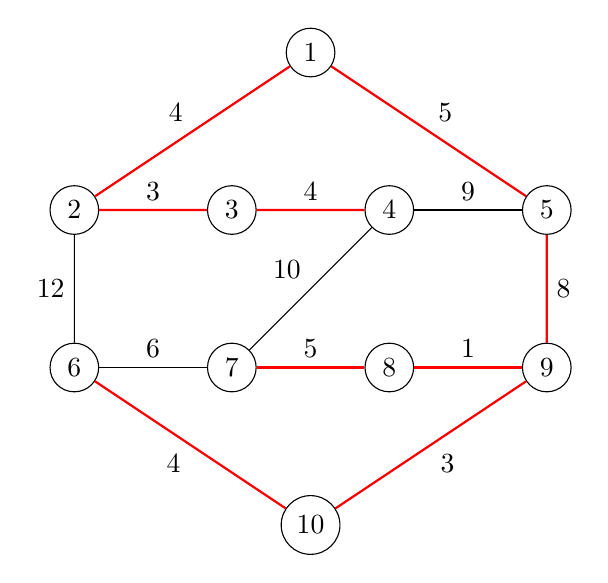
\begin{tikzpicture}
				\node[circle,draw=black, fill=white] (1) at (0,0) {1};
				\node[circle,draw=black, fill=white] (2) at (-3,-2) {2};
				\node[circle,draw=black, fill=white] (3) at (-1,-2) {3};
				\node[circle,draw=black, fill=white] (4) at (1,-2) {4};
				\node[circle,draw=black, fill=white] (5) at (3,-2) {5};
				\node[circle,draw=black, fill=white] (6) at (-3,-4) {6};
				\node[circle,draw=black, fill=white] (7) at (-1,-4) {7};
				\node[circle,draw=black, fill=white] (8) at (1,-4) {8};
				\node[circle,draw=black, fill=white] (9) at (3,-4) {9};
				\node[circle,draw=black, fill=white] (10) at (0,-6) {10};
				
				\draw (1) to node[above right] {5} (5) to node[right] {8} (9) to node[below right] {3} (10) to node[below left] {4} (6) to node[left] {12} (2) to node[above left] {4} (1);
				\draw (2) to node[above] {3} (3) to node[above] {4} (4) to node[above] {9} (5);
				\draw (6) to node[above] {6} (7) to node[above] {5} (8) to node[above] {1} (9);
				\draw (7) to node[above left] {10} (4);
				
				\draw[red,thick] (4) -- (3) -- (2) -- (1) -- (5) -- (9) -- (10) -- (6);
				\draw[red,thick] (9) -- (8) -- (7);
			\end{tikzpicture}
		\end{center}
		\item Es handelt sich um ein knotenorientiertes Problem. Da der Graph ungerichtet ist, ist dieses Problem ein symmetrisches TSP.
		\item 1 $\xrightarrow{4}$ 2 $\xrightarrow{3}$ 3 $\xrightarrow{4}$ 4 $\xrightarrow{9}$ 5 $\xrightarrow{8}$ 9 $\xrightarrow{1}$ 8 $\xrightarrow{4}$ 10 $\xrightarrow{4}$ 6 $\xrightarrow{6}$ 7 $\xrightarrow{19}$ 1, Gesamtlänge: 62
	\end{enumerate}

	\section*{Aufgabe 18}
	\begin{enumerate}[label=(\alph*)]
		\item Rundreiseproblem: 1 Tour, alle Ziele besuchen, keine Rückkehr zum Depot unterwegs \\
		Tourenproblem: mehrere Touren um alle Ziele zu besuchen, Rückkehr zum Depot nach einer Tour
		\item Hamilton-Tour: jeden Knoten genau einmal besuchen \\
		Euler-Tour: jede Kante genau einmal besuchen
		\item 1 $\xrightarrow{2}$ 3 $\xrightarrow{1}$ 2 $\xrightarrow{3}$ 4 $\xrightarrow{4}$ 5 $\xrightarrow{6}$ 1, Gesamtlänge: 16
	\end{enumerate}
	
\end{document}